\hypertarget{ux5377ux79efux795eux7ecfux7f51ux7edc}{%
\chapter{卷积神经网络}\label{ux5377ux79efux795eux7ecfux7f51ux7edc}}

\hypertarget{ux5377ux79efux795eux7ecfux7f51ux7edccnn}{%
\section{卷积神经网络（CNN）}\label{ux5377ux79efux795eux7ecfux7f51ux7edccnn}}

\hypertarget{ux4e00ux6838ux5fc3ux601dux60f3ux6a21ux4effux4ebaux7c7bux89c6ux89c9ux7684ux5c42ux6b21ux5316ux7279ux5f81ux63d0ux53d6}{%
\subsection{一、核心思想：模仿人类视觉的层次化特征提取}\label{ux4e00ux6838ux5fc3ux601dux60f3ux6a21ux4effux4ebaux7c7bux89c6ux89c9ux7684ux5c42ux6b21ux5316ux7279ux5f81ux63d0ux53d6}}

如识别一只猫：你首先注意到的是局部细节：边缘（胡须、耳朵轮廓）、斑点、颜色块。然后这些细节组合成更大的结构：眼睛、鼻子、爪子。最后，这些结构组合成整体概念：猫。

\hypertarget{ux4e8cux6838ux5fc3ux7ec4ux4ef6}{%
\subsection{二、核心组件}\label{ux4e8cux6838ux5fc3ux7ec4ux4ef6}}

\begin{enumerate}
\def\labelenumi{\arabic{enumi}.}
\tightlist
\item
  卷积层（Convolutional Layer）：特征探测器的滑动扫描
\end{enumerate}

（1）通俗解释

想象你拿一个放大镜（称为``滤波器''或``卷积核''）在图像上从左到右、从上到下慢慢滑动。这个放大镜有特殊能力，能``点亮''它看到的特定模式（比如垂直线、水平线、特定颜色）。它在每个位置都计算一个数值，表示该位置与放大镜关注模式的匹配程度。所有位置计算完后，你就得到了一张新的``特征图''，这张图突出了原始图像中符合该放大镜关注模式的所有区域。CNN 通常有很多个不同的放大镜（不同的滤波器），每个关注不同的模式（边缘、纹理、形状等），从而生成多张不同的特征图。

本质上，卷积核的每一个数值都是一些输入和一些输出之间的共同权重。输出单元只与输入的一个局部区域相连（感受野），而非全连接。同一个滤波器在输入的不同位置使用相同的权重。这意味着无论特征出现在图像的哪个位置，都由同一个探测器检测。这是 CNN 具有平移不变性（位置不变性）的基础，也是减少参数的核心。

（2）输入

每一次的输入是一个四维张量，按Pytorch的规则，第一个维度是batch\_size；第二个维度是input\_channels（输入通道数，如RGB图像第一个卷积层的输入通道数为3，代表3个颜色通道，后续卷积层的输入通道数则为前一层得到的特征数，卷积核的深度需与图像的通道数相同）；第三、四个维度是图像的高度和宽度input\_h和input\_w.

（3）卷积核

又称为滤波器，是一个小的、可学习的权重矩阵。滤波器矩阵有3个维度，分别为高度kernel\_h，宽度kernel\_w，通道数input\_channels。一个卷积层通常有多个滤波器，其个数即为输出通道数output\_channels。每个滤波器负责检测一种特定的局部空间模式，对应一个输出通道。

（4）卷积运算

输出矩阵是四维张量，第一个维度是batch\_size；第二个维度是output\_channels（卷积核个数）；第三、四个维度是output\_h和output\_w.

对于batch中的每一个样本：滤波器在输入上滑动（步长paddle），在每一个位置进行点积运算（Σ(卷积核的每一个元素*输入样本对应位置的元素)，然后再对各通道求和），然后可能还会加一个偏置，得到该样本该通道该位置的输出。

（5）卷积运算的底层实现

由于并行计算的效率远远高于用for循环，我们希望把卷积过程用矩阵乘法A\emph{B形式表征，A代表输入，B代表卷积核。由于输入是四维的、卷积核是三维的，我们会把部分维度合并展平。注意到矩阵乘法和点积的统一性，我们希望A的列数=B的行数=待点积的向量维度。容易发现这个待点积的向量维度是kernel\_h}kernel\_w*input\_channels，故构造A和B的行列如下：

A的行数=batch\_size（可以看成batch\_size个矩阵拼接）\emph{output\_h}output\_w（在多少个位置上进行卷积，即多少次卷积运算）

A的列数=B的行数=input\_channels\emph{kernel\_h}kernel\_w（卷积运算，按行、列、通道数求和）

B的列数=output\_channels（可以看成output\_channels个不同滤波器各自识别不同特征的矩阵拼接）

可以看出B就是权重矩阵，但A不是输入矩阵，而是需要对输入矩阵进行操作：

第b个样本，卷积核左上角在{[}i,j{]}，从输入矩阵里裁input\_data{[}b,i:i+kernel\_h,j:j+kernel\_w,:{]}，把这个矩阵展平，然后把所有这样的矩阵拼接。当然，为了加速，我们事实上往往会用unfold函数，对于每个卷积核中心可达的位置（行），都有其各个通道上``卷积核覆盖区''的所有kernel\_h\emph{kernel\_w个元素（列）,使用unfold提取图像块：第一步在维度2(高度)上用一个kernel\_h}1的``核''滑动，把这些元素``收集到核中心''，这时核中心可达位置有output\_h*input\_w个，结果形状：{[}batch\_size, input\_channels, output\_h, input\_w, kernel\_h{]}；第二步在维度3(宽度)上操作第一步得到的矩阵，结果形状：{[}batch\_size, input\_channels, output\_h, output\_w, kernel\_h, kernel\_w{]}。

有时还会加偏置，每个卷积核（每个输出通道）只有一个偏置。

\begin{enumerate}
\def\labelenumi{\arabic{enumi}.}
\setcounter{enumi}{1}
\tightlist
\item
  激活函数（Activation Function）：引入非线性
\end{enumerate}

卷积层计算出来的数值（特征匹配度）通常是线性的。但现实世界的数据和决策往往是高度非线性的。激活函数就像一个``开关''或``阈值处理器''，它决定一个特征是否足够强到被传递到下一层。它给网络增加了非线性的处理能力，使得网络能够学习复杂的映射关系。

\begin{enumerate}
\def\labelenumi{\arabic{enumi}.}
\setcounter{enumi}{2}
\tightlist
\item
  池化层（又称汇聚层，Pooling Layer）：降采样与空间信息压缩
\end{enumerate}

池化层就像一个``信息浓缩器''。它在一个小区域（比如 2x2 方块）内，选取一个代表值（比如最大值或平均值）。输入特征图，指定池化窗口大小P\_h*P\_w和步长S（通常等于窗口大小，即不重叠），窗口在输入特征图上按步长S滑动，在每个窗口区域内计算一个代表值，构成输出特征图。这个操作是逐通道独立进行的，没有需要学习的参数。

（1）池化操作分类

最大池化（Max Pooling）：取窗口内所有元素的最大值。

平均池化（Average Pooling）：取窗口内所有元素的平均值。

（2）池化操作的好处

降维（抓大放小）：汇聚层把特征图分成一个个小区域（如2x2像素），然后只从这个区域里选一个``代表''（最大值或平均值）。这就像把一张高分辨率照片缩略成小图，虽然细节少了，但猫的轮廓、主要特征还在。这极大减少后续层需要处理的数据量，降低计算成本和内存占用，防止网络过于复杂。

增强鲁棒性（位置不敏感）：如果图片里的猫稍微挪动了一点位置（平移几个像素），卷积层输出的特征位置会跟着变。但汇聚层只关心这个小区域里的``最强音''（最大值）或``整体调性''（平均值），只要这个区域里最强的特征还是猫耳朵，汇聚后的输出就能保持稳定。这使网络对目标的微小平移、旋转、缩放（尺度）变化更不敏感（即具有平移不变性），提高了模型的泛化能力。

防止过拟合（模糊细节）：通过丢弃精确的位置信息和一些非关键细节，降低了网络对训练数据中特定噪声或无关细节的敏感性，使模型更关注是否存在某种特征，而不是特征具体在哪个精确像素点。

扩大感受野（看得更广）：随着网络加深，后续的卷积层作用在汇聚后的特征图上，相当于能``看到''原始输入图像中更大的区域（更大的感受野），有助于捕捉更高层次的语义信息（如整个猫头而不是单根胡须）

（3）现代改进

可学习的汇聚参数：研究引入少量参数，让汇聚规则（如权重）能自适应学习，而非固定为~max~或~mean（如Learnable Power Pooling, SoftPool）。

结合注意力机制：利用注意力机制动态调整汇聚区域的重要性权重，更智能地选择或融合信息。

空洞卷积：通过增大卷积核的感受野（在元素间插入空洞）来避免使用汇聚层进行下采样，常用于需要高分辨率输出的任务（如语义分割）。

\begin{enumerate}
\def\labelenumi{\arabic{enumi}.}
\setcounter{enumi}{3}
\tightlist
\item
  全连接层（Fully Connected Layer）：综合决策
\end{enumerate}

在CNN的最后几层，经过多次卷积、激活、池化后得到的特征图（可能被展平成一维向量）会被送入一个或多个全连接层。这就像传统的神经网络（多层感知机MLP）。每个神经元都连接到前一层的所有神经元。它的作用是综合前面提取到的所有高级抽象特征，并根据这些特征做出最终的决策（比如这张图是``猫''还是``狗''的概率）。

\begin{enumerate}
\def\labelenumi{\arabic{enumi}.}
\setcounter{enumi}{4}
\tightlist
\item
  其他重要概念
\end{enumerate}

（1）填充（Padding）：在图像边缘周围添加一圈像素（通常是0），这样卷积时边缘信息也能被作为卷积区域的中心，从而让这些信息和中间信息得到``同等待遇''的卷积处理，控制输出特征图的大小不变。

（2）步长（Stride）：滤波器在水平和垂直方向上每次移动的像素数。步长越大，滑动越快，输出特征图越小，感受野增加越快。

（3）批归一化（Batch Normalization）：在训练过程中，对每一层（通常在卷积层或全连接层之后，激活函数之前）的输入进行归一化处理（减均值除标准差），并引入可学习的缩放和平移参数。这能加速训练、缓解梯度消失/爆炸、允许使用更高的学习率、有一定的正则化效果。

对于一个 mini-batch 的输入 \(B=\{x_1,\ldots,x_m\}\)，计算 mini-batch 均值和方差：

\[
\mu_B=\frac{1}{m}\sum_{i=1}^{m}x_i,\qquad
\sigma_B^2=\frac{1}{m}\sum_{i=1}^{m}(x_i-\mu_B)^2
\]

归一化与缩放平移为：

\[
\hat{x}_i=\frac{x_i-\mu_B}{\sqrt{\sigma_B^2+\epsilon}},\qquad
y_i=\gamma\hat{x}_i+\beta
\]

其中 \(\epsilon\) 是小的常数，用于防止除零；\(\gamma\) 和 \(\beta\) 是可学习参数，用于恢复网络的表达能力。

（4）Dropout：在训练时，随机让一部分神经元暂时``失效''（输出置零）。这迫使网络不能过分依赖某些特定的神经元，增强了模型的泛化能力，减少过拟合。训练时，对每个神经元以概率p将其输出置零。测试时，所有神经元都激活，但输出值要乘以1-p（或训练时乘以1/(1-p)，测试时不变）以保持期望输出值不变。

\begin{enumerate}
\def\labelenumi{\arabic{enumi}.}
\setcounter{enumi}{5}
\tightlist
\item
  多通道（Multi-Channel）
\end{enumerate}

事实上，输入数据或特征图不是一个单一的二维矩阵（H\emph{W），而是一个三维张量：H(Height) }W(Width)*C(Channels)。

对于输入图像，一个标准的RGB彩色图像的输入为H\emph{W}3矩阵，有3个通道：红色通道（R）、绿色通道（G）、蓝色通道（B）。每个通道都是一个二维网格（矩阵），网格中的每个值（像素）表示该位置对应颜色（R/G/B）的强度。灰度图像只有1个通道（亮度）。

对于在CNN的卷积层之后产生的特征图，其通道数表示不同类型的特征。例如，第一个卷积层输出的某个通道可能主要对``垂直边缘''敏感，另一个通道可能对``45度边缘''或``红色区域''敏感。随着网络加深，通道代表的特征越来越抽象（如``车轮''、``猫耳朵''的某种模式）。某个卷积层输出的特征图的尺寸为H\emph{W}C\_out，输出通道数C\_out是该层使用的卷积核的数量，也就是不同类型特征的个数。

在位置(i, j)使用卷积核进行卷积的操作分为如下步骤：

（1）提取输入块：在输入X上，取出一个与卷积核大小相同的三维块X{[}i:i+K\_h, j:j+K\_w, :{]}。这个块的维度是(K\_h, K\_w, C\_in)。输入通道与卷积核深度必须相等（都为C\_in），这是多通道卷积能融合不同通道信息的基础。卷积核在通道维度上``扫描''并整合所有输入通道的信息。

（2）逐通道点积并求和：将卷积核与这个输入块进行逐元素相乘，得到一个同样大小的三维结果块(K\_h, K\_w, C\_in)。例如，在RGB输入中，一个检测``红色物体边缘''的卷积核，可能会在R通道赋予正权重，在G和B通道赋予负权重或零权重；在深层特征图中，一个检测``车轮''的卷积核，可能会组合来自不同底层特征通道（如``圆形''、``黑色区域''、``纹理''）的信息。。

（3）全局求和并加偏置：将上一步得到的三维结果块中的所有元素相加，加上一个标量偏置项b\_k（这个偏置是每个卷积核独有的）。这将卷积核在每个空间位置、每个输入通道上计算的相关性汇总成一个标量值。这个标量值代表了该卷积核所检测的特定特征（如某种边缘、纹理、颜色组合）在当前位置(i, j)的综合响应强度。

（4）得到输出值：这个(Sum + b\_k)的值，就是输出特征图O在位置(i, j)，对应第k个卷积核（即输出通道k）的值：O{[}i, j, k{]} = b\_k + sum\_\{di=0\}\^{}\{K\_h-1\} sum\_\{dj=0\}\^{}\{K\_w-1\} sum\_\{c=0\}\^{}\{C\_in-1\} ( X{[}i+di, j+dj, c{]} * K{[}di, dj, c, k{]} )。

\hypertarget{ux4e09ux5178ux578bux67b6ux6784ux6a21ux5f0f}{%
\subsection{三、典型架构模式}\label{ux4e09ux5178ux578bux67b6ux6784ux6a21ux5f0f}}

经典的 CNN 架构通常遵循以下模式：

输入图像 -\textgreater{} {[} {[}卷积层 -\textgreater{} 激活函数{]} * N -\textgreater{} 池化层 {]} * M -\textgreater{} 展平层 -\textgreater{} {[}全连接层 -\textgreater{} 激活函数{]} * K -\textgreater{} 输出层

随着层数加深，空间分辨率逐渐降低（池化、大步长卷积），通道数逐渐增加（使用更多不同的滤波器），提取的特征从低级（边缘、角点、纹理）向高级（物体部件、完整物体、场景）演变。最后全连接层将提取到的高级特征进行整合，完成最终任务（分类、回归等）。

经典卷积神经网络示例：LeNet

LeNet-5（经典版本）由 7 层组成，输入为 \(32\times 32\) 灰度图像，输出为 0-9 数字的概率分布：

\begin{longtable}[]{@{}
  >{\raggedright\arraybackslash}p{(\columnwidth - 8\tabcolsep) * \real{0.20}}
  >{\raggedright\arraybackslash}p{(\columnwidth - 8\tabcolsep) * \real{0.20}}
  >{\raggedright\arraybackslash}p{(\columnwidth - 8\tabcolsep) * \real{0.20}}
  >{\raggedright\arraybackslash}p{(\columnwidth - 8\tabcolsep) * \real{0.20}}
  >{\raggedright\arraybackslash}p{(\columnwidth - 8\tabcolsep) * \real{0.20}}@{}}
\toprule
层名称 & 操作 & 输入尺寸 & 输出尺寸 & 核心作用 \\
\midrule
\endhead
输入层 & 原始图像 & \(32\times 32\times 1\) & \(32\times 32\times 1\) & 接收灰度图像 \\
C1卷积层 & 6 个 \(5\times 5\) 卷积核 & \(32\times 32\times 1\) & \(28\times 28\times 6\) & 提取边缘/纹理特征 \\
S2池化层 & \(2\times 2\) 平均池化 & \(28\times 28\times 6\) & \(14\times 14\times 6\) & 降维，保留关键特征 \\
C3卷积层 & 16 个 \(5\times 5\) 卷积核 & \(14\times 14\times 6\) & \(10\times 10\times 16\) & 提取复杂特征（如数字局部结构） \\
S4池化层 & \(2\times 2\) 平均池化 & \(10\times 10\times 16\) & \(5\times 5\times 16\) & 进一步降维 \\
C5全连接层 & 展平 + 全连接 & \(5\times 5\times 16\rightarrow 400\) & 120 & 综合高级特征 \\
F6全连接层 & 全连接 & 120 & 84 & 非线性特征映射 \\
输出层 & 全连接 + Softmax & 84 & 10 & 生成分类概率 \\
\bottomrule
\end{longtable}

\hypertarget{ux56dbcnnux7684ux4f18ux52bf}{%
\subsection{四、CNN的优势}\label{ux56dbcnnux7684ux4f18ux52bf}}

\begin{enumerate}
\def\labelenumi{\arabic{enumi}.}
\item
  参数共享：同一个滤波器在整个图像上滑动使用相同的权重，极大减少了需要学习的参数数量（与全连接网络相比）。这使得训练更高效，模型更小，需要的训练数据相对更少，且具有平移不变性。
\item
  局部连接：输出单元只与输入的一个局部区域连接，这符合图像数据的局部相关性特性（像素的语义通常由其邻近像素决定），也减少了参数。
\item
  层次化特征提取：自动从原始像素开始学习越来越复杂的特征（边缘 -\textgreater{} 纹理 -\textgreater{} 部件 -\textgreater{} 物体），无需人工设计特征。
\item
  平移不变性：由于参数共享和池化操作，网络对目标在图像中的位置变化具有一定的不敏感性。特征出现在哪里不重要，重要的是它出现了。
\item
  空间层次性：网络结构自然地通过卷积和池化操作建立了空间上的层次结构。
\end{enumerate}

\hypertarget{ux4e94ux5377ux79efux795eux7ecfux7f51ux7edcux7684ux67b6ux6784ux53d8ux5316ux8d8bux52bf}{%
\subsection{五、卷积神经网络的架构变化趋势}\label{ux4e94ux5377ux79efux795eux7ecfux7f51ux7edcux7684ux67b6ux6784ux53d8ux5316ux8d8bux52bf}}

\begin{enumerate}
\def\labelenumi{\arabic{enumi}.}
\item
  减少池化层，用步长大于1的卷积代替降采样。
\item
  大量使用批量归一化层。
\item
  使用更深的网络（ResNet, DenseNet等通过跳跃连接解决深度网络训练难题）。
\item
  使用更小的滤波器（如3x3卷积堆叠代替大卷积核）。
\end{enumerate}

\hypertarget{ux53c2ux8003ux6587ux732e-9}{%
\subsection{参考文献}\label{ux53c2ux8003ux6587ux732e-9}}

\begin{itemize}
\tightlist
\item
  LeCun, Y., Bottou, L., Bengio, Y., \& Haffner, P. (1998). \href{http://yann.lecun.com/exdb/publis/pdf/lecun-98.pdf}{Gradient-Based Learning Applied to Document Recognition}. Proceedings of the IEEE.
\item
  Krizhevsky, A., Sutskever, I., \& Hinton, G. E. (2012). \href{https://papers.nips.cc/paper/4824-imagenet-classification-with-deep-convolutional-neural-networks}{ImageNet Classification with Deep Convolutional Neural Networks}. NeurIPS 2012.
\end{itemize}

\clearpage

\hypertarget{nin}{%
\section{NiN}\label{nin}}

\hypertarget{ux4e00ux6838ux5fc3ux601dux60f3ux7528ux5faeux7f51ux7edcux589eux5f3aux7279ux5f81ux62bdux8c61ux80fdux529b}{%
\subsection{一、核心思想：用``微网络''增强特征抽象能力}\label{ux4e00ux6838ux5fc3ux601dux60f3ux7528ux5faeux7f51ux7edcux589eux5f3aux7279ux5f81ux62bdux8c61ux80fdux529b}}

传统CNN的卷积操作本质是点积，这是线性的。在每一步卷积后，高级特征和每一个低级特征都有一个线性相关系数（外加一个激活函数，但只经过一次激活其实对相关性影响没那么大），但如果高级特征和低级特征之间严重不符合这种关系，就会出现较大偏差。

NiN的做法是，在每一步卷积操作后再加入参数量较小的全连接网络（多层感知机，MLP），这样就会经过多次激活，这个全连接网络的输出（高级特征）和输入（低级特征）也就不会是只有一个参数（卷积核参数）的线性关系，整体处理非线性关系的能力较强。

\hypertarget{ux4e8cux6838ux5fc3ux7ec4ux4ef6-1}{%
\subsection{二、核心组件}\label{ux4e8cux6838ux5fc3ux7ec4ux4ef6-1}}

\begin{enumerate}
\def\labelenumi{\arabic{enumi}.}
\tightlist
\item
  MLP卷积层
\end{enumerate}

结构：一个MLP卷积层会在常规卷积后，再引入多个（通常是两个左右）1x1卷积层。

1x1卷积的作用不是在长x宽空间上融合信息（因为空间上是1x1），而是重构各个通道，``改变通道数''。具体地说，我们知道，卷积层的输入是分通道的（色彩通道或低级特征），输出也是分通道的（高级特征），每个输入通道和每个输出通道之间有连结（准确说输出通道的数值参考了各输入通道数值的加权），因此1x1卷积等价于对于每个像素而言，各输入通道与各输出通道间建立全连接层。

每个1x1卷积层后接一个非线性激活函数（如ReLU）。

数学表达（以传统卷积层+一个额外的1x1卷积层为例）：

对于一个输入局部块x（例如一个3x3xc的区域），传统卷积输出是y = σ(w · x + b)（σ是激活函数，如ReLU）。

而一个两层的MLP卷积输出是y =σ₂( W₂·(σ₁( W₁·x + b₁)) + b₂)，其中W₁, W₂是可学习的权重矩阵（即1x1卷积核），b₁, b₂是偏置。因为增加了一个矩阵，这明显是一个更复杂的非线性函数，也能处理更复杂的非线性特征关系。

参数高效：即使堆叠多个1x1卷积，参数量也远小于使用大尺寸的卷积核。

\begin{enumerate}
\def\labelenumi{\arabic{enumi}.}
\setcounter{enumi}{1}
\tightlist
\item
  全局平均池化（Global Average Pooling，GAP）
\end{enumerate}

这是NiN另一个极具影响力的贡献，旨在取代传统的全连接层。

传统CNN的问题：在NiN之前，CNN的末端通常使用一个或多个全连接层来进行分类。FC层参数量巨大（占整个网络参数的90\%以上），极易导致过拟合，并且破坏了特征图的空间结构信息。NiN的解决方案（GAP）通过修改池化层直接代替了参数庞大的全连接层。

（1）假设NiN最后一个MLP卷积层输出的特征图尺寸是。其中c可以直接设置为``对目标分类的类别数''（例如，ImageNet有1000类，则c=1000）。

（2）对这张特征图的每一个通道，计算其所有个像素的平均值。

（3）这样，每个通道都会产生一个标量值。c个通道就产生一个c维的向量。直接将这个c维向量送入Softmax层，即可得到每个类别的概率分布。

优势：

（1）极大减少参数，防止过拟合：GAP完全没有需要学习的参数，使模型更小、更不容易过拟合。

（2）更符合卷积精神：它将整个网络保持为卷积结构，输入可以是任意尺寸（因为GAP操作对输入尺寸没有要求）。

（3）显式地赋予特征图语义：每个最终的特征图通道都可以被直观地解释为``对应某个类别的置信度图''，该通道全局平均代表``为该类别的平均置信度''。

\begin{enumerate}
\def\labelenumi{\arabic{enumi}.}
\setcounter{enumi}{2}
\tightlist
\item
  一个典型的NiN网络（如用于CIFAR-10的NiN）结构如下：
\end{enumerate}

Input -\textgreater{}

{[}MLPConv Layer (e.g., 192x5x5 -\textgreater{} 160x1x1 -\textgreater{} 96x1x1){]} -\textgreater{} Max Pooling -\textgreater{}

{[}MLPConv Layer (e.g., 192x5x5 -\textgreater{} 192x1x1 -\textgreater{} 192x1x1){]} -\textgreater{} Max Pooling -\textgreater{}

{[}MLPConv Layer (e.g., 192x3x3 -\textgreater{} 192x1x1 -\textgreater{} 10x1x1){]} -\textgreater{}

Global Average Pooling (to 10x1x1) -\textgreater{}

Softmax

注：（1）它交替堆叠MLP卷积层和最大池化层。

（2）越靠后的层，特征图空间尺寸越小，通道数越多。

（3）最后一级的MLPConv层，其输出通道数直接设置为类别数（如10）。最终通过``全局平均池化''得到分类结果。

\hypertarget{ux53c2ux8003ux6587ux732e-10}{%
\subsection{参考文献}\label{ux53c2ux8003ux6587ux732e-10}}

\begin{itemize}
\tightlist
\item
  Lin, M., Chen, Q., \& Yan, S. (2013). \href{https://arxiv.org/abs/1312.4400}{Network In Network}. arXiv:1312.4400.
\end{itemize}

\clearpage

\hypertarget{googlenet}{%
\section{GoogLeNet}\label{googlenet}}

\hypertarget{ux4e00ux6838ux5fc3ux521bux65b0inception-ux6a21ux5757}{%
\subsection{一、核心创新：Inception 模块}\label{ux4e00ux6838ux5fc3ux521bux65b0inception-ux6a21ux5757}}

这是GoogLeNet的灵魂。其设计目标是在多个尺度上同时处理特征，并让网络自动学习选择最合适的尺度。

\begin{enumerate}
\def\labelenumi{\arabic{enumi}.}
\tightlist
\item
  Naïve Inception 模块（原始想法）
\end{enumerate}

最初的设想很简单：与其纠结于使用1x1、3x3还是5x5卷积核，或者要不要池化，不如让网络自己选择！在一个局部区域，并行地应用多种类型的操作，然后将所有结果在通道维度上拼接（Concatenate）~起来，形成输出。

结构如下：
一个输入同时送入4个并行分支：

1x1 卷积：~用于捕获极局部的特征，也是一种线性投影。

3x3 卷积：~捕获稍大一些的区域特征。

5x5 卷积：~捕获更大范围的感受野。

3x3 最大池化：~提取最显著的特征，提供空间上的鲁棒性。

所有分支的输出特征图（确保它们的高度和宽度相同）在通道维度上堆叠在一起，作为本模块的最终输出。

核心问题：计算量爆炸！
5x5卷积的计算成本已经很高，而每个分支都会产生大量输出通道。直接将所有分支的输出（可能成百上千个通道）拼接起来，会导致输出通道数急剧增加，并给下一个Inception模块带来巨大的计算负担。这个``天真''的设计在计算上是不可行的。

\begin{enumerate}
\def\labelenumi{\arabic{enumi}.}
\setcounter{enumi}{1}
\tightlist
\item
  真正的 Inception 模块（with Dimension Reduction）
\end{enumerate}

GoogLeNet论文的神来之笔是为这些并行分支引入了~``瓶颈层''------即1x1卷积，用它来降维，从而显著降低计算成本。

1x1卷积的核心作用：

（1）跨通道信息整合与降维：~在进入昂贵的3x3或5x5卷积之前，先用1x1卷积减少通道数。例如，将256个通道先压缩到64个，再进行3x3卷积，计算量会大幅下降。

（2）增加非线性：~每个1x1卷积后都跟随一个ReLU激活函数，增强了模型的非线性表达能力。改进后的Inception模块结构：

1x1卷积分支：~保留不变。

3x3卷积分支：~在3x3卷积之前，先通过一个1x1卷积进行降维。

5x5卷积分支：~在5x5卷积之前，先通过一个1x1卷积进行降维。

池化分支：~在3x3最大池化之后，通过一个1x1卷积进行降维。这一点至关重要，因为池化操作不会改变通道数，如果不进行降维，池化分支的输出通道数将与输入相同，拼接后仍然会导致通道数膨胀。

\hypertarget{ux4e8cux7ecfux5178ux67b6ux6784}{%
\subsection{二、经典架构}\label{ux4e8cux7ecfux5178ux67b6ux6784}}

\begin{enumerate}
\def\labelenumi{\arabic{enumi}.}
\tightlist
\item
  主干网络 (Stem Network)
\end{enumerate}

这是网络的开头部分，由一些传统的卷积层和最大池化层组成，负责进行基础的底层特征提取和快速降采样。

作用：~快速将输入图像的高度和宽度缩小，同时增加通道数，为后面大量的Inception模块处理做准备。

具体操作：~输入（224x224x3）经过一系列7x7卷积（步幅2）、ReLU、最大池化、3x3卷积（步幅1）、ReLU等操作，迅速将空间尺寸压缩，并提升通道数。

\begin{enumerate}
\def\labelenumi{\arabic{enumi}.}
\setcounter{enumi}{1}
\tightlist
\item
  Inception 模块的堆叠
\end{enumerate}

主干网络之后，网络进入了多个连续的Inception模块组。每组之间由最大池化层进行降采样，空间尺寸（高和宽）减半，通道数增加。

Inception (3a), (3b):~位于第一个池化层之后，是网络中较浅的Inception模块。

Inception (4a), (4b), (4c), (4d), (4e):~位于第二个池化层之后，是网络中间部分的核心模块。注意，两个辅助分类器就挂载在4a和4d的输出之上。

Inception (5a), (5b):~位于最后一个池化层之后，是网络最深层的模块，处理最抽象的特征。

\begin{enumerate}
\def\labelenumi{\arabic{enumi}.}
\setcounter{enumi}{2}
\tightlist
\item
  辅助分类器 (Auxiliary Classifiers)
\end{enumerate}

这是GoogLeNet另一个非常巧妙的设计，用来解决梯度消失问题，尤其是在如此深的网络中。

动机：~深度网络在训练时，梯度反向传播到浅层时会变得非常小，导致浅层的权重更新缓慢，难以训练。这被称为梯度消失。

结构：~在网络中间层（4a和4d的输出后）添加两个小型的、完整的分类器：

一个平均池化层（5x5，步幅3）进行降维。

一个1x1卷积（128通道）进一步压缩通道数。

两个全连接层（1024个单元）。

Dropout层（70\%保留）防止过拟合。

一个Softmax分类输出层（1000类）。

作用：

反向传播梯度：~在训练阶段，辅助分类器会根据中间层的特征做出预测，并计算损失。这个损失会乘以一个较小的权重（如0.3）后直接反向传播到浅层，为浅层提供``更清晰''、更强的梯度信号，极大地缓解了梯度消失问题，确保了整个网络都能得到充分训练。

正则化效果：~辅助分类器迫使中间层也能学习到有判别性的特征，起到了正则化的作用，一定程度上防止过拟合。

说明：在测试和实际使用时，辅助分类器会被完全丢弃，不会参与前向传播。因此，它不会增加最终的推理时间。

\begin{enumerate}
\def\labelenumi{\arabic{enumi}.}
\setcounter{enumi}{3}
\tightlist
\item
  分类输出层
\end{enumerate}

全局平均池化：~在经过所有Inception模块后，网络使用全局平均池化（GAP）~来替代传统的全连接层。它将最后一个Inception模块（5b）输出的~7x7x1024~的特征图每个通道全部取平均值，直接得到一个1024维的向量。这彻底移除了全连接层，极大减少了参数量（从数百万降到1024），有效控制了过拟合。

Dropout：~在GAP之后，仍然使用了Dropout（40\%丢弃率）作为正则化手段。

线性层 + Softmax：~最后是一个简单的线性层（将1024维向量映射到1000维）和Softmax激活函数，输出1000个类的概率分布。

\begin{enumerate}
\def\labelenumi{\arabic{enumi}.}
\setcounter{enumi}{4}
\tightlist
\item
  为什么主干网络不用Inception？
\end{enumerate}

（1）任务不同：低级特征 vs.~高级特征

主干网络的任务：~处理原始输入图像（RGB像素）。它的核心目标是快速提取最基础、最通用的低级特征，如边缘、角点、颜色块、纹理等。这些特征非常简单，不需要复杂的、多尺度的融合来判断。一个简单的、相对大一点的卷积核（如7x7）就能有效地捕获这些局部模式。

Inception模块的任务：~处理已经过初步处理的特征图。它的核心目标是对这些基础特征进行组合、抽象和筛选，以形成更高级、更复杂的特征，如``车轮''、``眼睛''、``纹理组合''等。这时才需要``多路径''并行的设计来让网络选择是用1x1、3x3还是5x5的变换更有效。

（2）计算效率：避免在计算成本最高的地方增加开销

输入图像的空间尺寸是最大的，但通道数是最少的（只有3个通道）。

计算成本分析：~卷积操作的计算量与输入特征图的尺寸（H x W）~和通道数（C\_in）~直接相关。在网络最开端，H和W很大（例如224x224），但C\_in很小（3）。

如果在此使用Inception：多分支结构意味着需要并行计算多个卷积操作，然后将结果拼接。这种并行性在开局阶段会带来巨大的计算负担，但收益甚微（因为只是提取低级特征）。

使用传统层的优势：

一个7x7卷积（步幅2）~可以非常高效地在一层内实现大幅降采样（图像尺寸快速减半）和底层特征提取。接着跟一个最大池化层，进一步快速降低空间尺寸。这样只用一两层就迅速将数据量降下来，为后面更深、更复杂的Inception模块扫清了计算障碍。

结论：在计算成本最高的输入阶段保持结构简单，是优化整体网络效率的关键策略。

（3）信息保留：过早的并行拼接可能造成干扰

在网络的最开始，信息是高度密集且未被处理的原始像素。过早地引入多路径并对其进行拼接（Concatenation），可能会将一些不相关的、冗余的低级信息混合在一起，反而为网络后续的处理增加噪音。

\hypertarget{ux4e09googlenet-ux7684ux610fux4e49ux4e0eux5f71ux54cd}{%
\subsection{三、GoogLeNet 的意义与影响}\label{ux4e09googlenet-ux7684ux610fux4e49ux4e0eux5f71ux54cd}}

开创了模块化设计先河：~GoogLeNet证明了通过精心设计一个小的基础模块（Inception），然后像搭乐高一样堆叠它，可以构建出非常强大且高效的网络。这种思想被后续几乎所有现代网络架构所采用（如ResNet, DenseNet）。

极致的高效性：~在取得顶级精度的同时，参数量仅为500万左右（AlexNet的1/12，VGG的1/27），计算量也更低，展示了卓越的性能-计算比。

\hypertarget{ux53c2ux8003ux6587ux732e-11}{%
\subsection{参考文献}\label{ux53c2ux8003ux6587ux732e-11}}

\begin{itemize}
\tightlist
\item
  Szegedy, C., Liu, W., Jia, Y., et al.~(2015). \href{https://arxiv.org/abs/1409.4842}{Going Deeper with Convolutions}. CVPR 2015.
\end{itemize}

\clearpage

\hypertarget{ux6b8bux5deeux7f51ux7edcresnet}{%
\section{残差网络（ResNet）}\label{ux6b8bux5deeux7f51ux7edcresnet}}

\hypertarget{ux4e00ux6838ux5fc3ux601dux60f3ux8ba9ux7f51ux7edcux5b66ux4e60ux6b8bux5deeux800cux975eux539fux59cbux6620ux5c04}{%
\subsection{一、核心思想：让网络学习``残差''而非``原始映射''}\label{ux4e00ux6838ux5fc3ux601dux60f3ux8ba9ux7f51ux7edcux5b66ux4e60ux6b8bux5deeux800cux975eux539fux59cbux6620ux5c04}}

\begin{enumerate}
\def\labelenumi{\arabic{enumi}.}
\tightlist
\item
  问题：深度网络的困境
\end{enumerate}

在ResNet之前，人们发现一个反直觉的现象：单纯地增加网络深度，反而会导致性能下降。这不仅是测试集上的过拟合，训练误差也会随之增大。这意味着，更深的网络甚至更难优化（harder to train）。这个问题被称为网络退化（Degradation Problem）。

梯度消失/爆炸：~虽然通过Batch Normalization等技术可以很大程度上缓解，但并非完全根除。

网络退化：~即使解决了梯度问题，56层的网络性能反而比20层的网络更差。这表明，深网络并非天生就难以训练，而是现有的优化算法难以找到那些理论上应该存在的、更优的解。

\begin{enumerate}
\def\labelenumi{\arabic{enumi}.}
\setcounter{enumi}{1}
\tightlist
\item
  解决方案：跳跃连接（Skip Connection / Shortcut）
\end{enumerate}

ResNet的解决方案非常简洁而有力：如果深层网络难以学习到理想的映射~H(x)，那么我们就让它去学习这个映射与输入~x~之间的残差（Residual）F(x) = H(x) - x。

原始映射：~H(x) = x~（恒等映射）
残差映射：~F(x) = H(x) - x
目标映射重构：~H(x) = F(x) + x

为什么学习原始映射比残差映射更难：残差映射总体接近0，目标映射总体接近x。我们知道，让一个充满各种求和以及激活函数的神经网络去拟合y=x并不容易，但拟合y=0只需要所有参数都趋近0即可。

概率论角度：ResNet为网络提供了一个``恒等映射''的先验（默认捷径）。这时候，学习一个相对于恒等映射的``小扰动''或``小修正''~F(x)，远比学习一个全新的复杂映射~H(x)~要容易得多。

最坏情况：学不到残差分布，直接变成H(x) = x，也就是残差块输出=残差块输入（注意残差块不代表整个神经网络），比如一个两层神经网络，残差块在第二层，最差的结果是相当于这层什么也不做，直接退化为一层。但如果不用残差网络，可能出现连H(x) ≈x的主要特征都学不到，性能还不如只有一层的情况。

通俗比喻：
假设你要学习从北京到上海的路线（映射~H(x)）。

传统网络：~需要从头开始学习整个路线，容易迷路或走错。

ResNet：~你 already know 一条主线高速公路（即输入~x）。你只需要学习从主线上的一些匝道出去，去探索一些新的小路，然后再回到主线上。你的任务是学习这些``匝道和小路''的修正量（即残差~F(x)）。即使你探索的小路是死胡同（F(x) = 0），你依然可以退回到主线高速上（H(x) = x），保证性能不会比原来的主线更差。这大大降低了学习的风险和难度。

在网络上，这个``回到主线''的操作就是通过跳跃连接（Shortcut Connection）~实现的，它直接将输入~x~跳过多层，加到这几层的输出~F(x)~上。

从函数类的角度看，ResNet 的关键优势在于让更深网络的函数类尽量形成``嵌套''关系。

\begin{itemize}
\tightlist
\item
  嵌套函数类（Nested Function Classes）：例如 \(\mathcal{F}_1\)（1 层网络）\(\subseteq \mathcal{F}_2\)（2 层网络）\(\subseteq \cdots \subseteq \mathcal{F}_6\)（6 层网络）。这意味着 2 层网络完全可以模拟 1 层网络的行为，只需要让第二层什么都不做即可。
\item
  非嵌套函数类（Non-Nested Function Classes）：如果更复杂的网络结构不能包含简单结构，例如 \(\mathcal{F}_6\) 是一种与 \(\mathcal{F}_1\) 完全不同的架构，那么就没有任何保证。更复杂的网络可能反而学得更差，因为它可能根本学不到简单网络已经找到的好解。
\end{itemize}

通俗比喻：想象你要造更快的车。

\begin{itemize}
\tightlist
\item
  嵌套：新款赛车（\(\mathcal{F}_2\)）是在旧款赛车（\(\mathcal{F}_1\)）的基础上改装升级引擎。它至少和旧款一样快，甚至更快。
\item
  非嵌套：新款赛车（\(\mathcal{F}_6\)）被设计成了一艘船。它可能在水里更快，但在陆地上（图像分类任务上）反而比旧款赛车慢得多。
\end{itemize}

\hypertarget{ux4e8cux6b8bux5deeux5757ux67b6ux6784}{%
\subsection{二、残差块架构}\label{ux4e8cux6b8bux5deeux5757ux67b6ux6784}}

\begin{figure}[htbp]
\centering
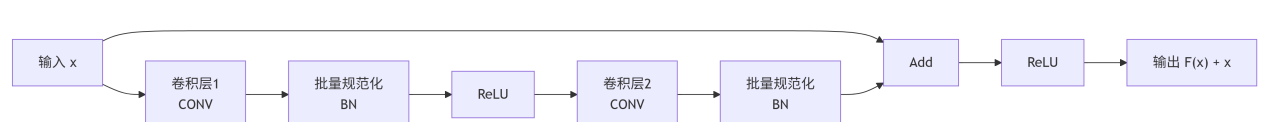
\includegraphics{images/image-0007.png}
\caption{ResNet 残差块结构}
\end{figure}

注意：F(x) + x~是逐元素相加（Element-wise Addition），意味着~F(x)~的输出必须与~x~的维度完全相同。这要求残差块内的最后一层卷积必须将通道数调整到与~x~一致。

ResNet通过堆叠上述残差块构建了不同深度的网络。

\hypertarget{ux4e09ux6b8bux5deeux7f51ux7edcux4e3aux4f55ux5982ux6b64ux6709ux6548}{%
\subsection{三、残差网络为何如此有效？}\label{ux4e09ux6b8bux5deeux7f51ux7edcux4e3aux4f55ux5982ux6b64ux6709ux6548}}

\begin{enumerate}
\def\labelenumi{\arabic{enumi}.}
\item
  解决梯度消失问题：~跳跃连接提供了一条``高速公路''，使得梯度可以从深层几乎无损耗地、直接地反向传播到浅层。这使得超深度网络的训练成为可能。
\item
  简化学习目标：~学习残差~F(x) = H(x) - x~通常比学习完整的映射~H(x)~更容易。特别是，当``恒等映射''已经是最优或接近最优时，将残差~F(x)~推近0比用一堆非线性层去拟合一个恒等映射要容易得多。
\item
  隐式的模型集成：~有理论认为，ResNet的行为类似于一个众多浅层网络的集成。由于跳跃连接的存在，数据可以沿不同深度的路径流动，使得网络同时具有浅层和深层的特性。
\end{enumerate}

\hypertarget{ux56dbux53d8ux4f53}{%
\subsection{四、变体}\label{ux56dbux53d8ux4f53}}

瓶颈结构（Bottleneck）：~为了在更深的网络（如ResNet-50/101/152）中减少计算量，每个残差块内采用了``瓶颈''设计：1x1卷积（降维） -\textgreater{} 3x3卷积 -\textgreater{} 1x1卷积（升维）。这大大减少了3x3卷积的计算开销。

\hypertarget{ux4e94ux73b0ux4ee3ux5927ux6a21ux578bux4e2dux6b8bux5deeux7684ux5e94ux7528}{%
\subsection{五、现代大模型中残差的应用}\label{ux4e94ux73b0ux4ee3ux5927ux6a21ux578bux4e2dux6b8bux5deeux7684ux5e94ux7528}}

现代大模型中，不是用一个从输入直接连到输出的残差一般在每个块或层中，都会加一个残差结构，以让梯度和信息顺畅流过该块或层，使信息流动更灵活，如 Transformer 架构里的多处 Add。

\hypertarget{ux53c2ux8003ux6587ux732e-12}{%
\subsection{参考文献}\label{ux53c2ux8003ux6587ux732e-12}}

\begin{itemize}
\tightlist
\item
  He, K., Zhang, X., Ren, S., \& Sun, J. (2016). \href{https://arxiv.org/abs/1512.03385}{Deep Residual Learning for Image Recognition}. CVPR 2016.
\end{itemize}

\clearpage

\hypertarget{densenet}{%
\section{DenseNet}\label{densenet}}

在ResNet中，我们看到了跳跃连接（x + F(x)）的巨大威力。DenseNet的作者提出了一个更激进的想法：为了最大化网络中各层之间的信息流动，能否让每一层都直接连接到它后面的所有层？

在这种连接模式下，每一层都从所有 preceding layers（前面的层）中接收``集体知识''作为输入，并将其自身的特征图传递给所有 subsequent layers（后面的层）。

\hypertarget{ux4e00ux6838ux5fc3ux7ec4ux4ef6ux5bc6ux96c6ux5757dense-blockux4e0eux8fc7ux6e21ux5c42transition-layer}{%
\subsection{一、核心组件：密集块（Dense Block）与过渡层（Transition Layer）}\label{ux4e00ux6838ux5fc3ux7ec4ux4ef6ux5bc6ux96c6ux5757dense-blockux4e0eux8fc7ux6e21ux5c42transition-layer}}

DenseNet的结构由两种核心模块交替组成。

\begin{enumerate}
\def\labelenumi{\arabic{enumi}.}
\tightlist
\item
  密集块（Dense Block）
\end{enumerate}

密集块是DenseNet的核心构建单元。在一个密集块内部，每一层都直接与块内的所有后续层相连。

数学表达：设第~l~层的输出为~x\_l，则第~l~层的输入是前面所有层输出的拼接（Concatenation）：x\_l = H\_l({[}x\_0, x\_1, \ldots, x\_\{l-1\}{]})
其中~{[} \ldots{} {]}~表示在通道维度（Channel Dimension）~上进行拼接，H\_l(·)~代表一个复合函数（如BN-ReLU-Conv）。

结构剖析：

复合函数~H\_l：~通常是一个标准的序列，包括批量规范化（BN）、ReLU激活函数~和~3x3卷积（Conv）。这个3x3卷积通常只产生很少的特征图（例如~k=32~个），这个数字~k~被称为增长率（Growth Rate）。

拼接操作：~每一层都会将其输出的~k~个特征图添加到整个块的``集体知识''中。因此，越靠后的层，其输入通道数会越多（因为它拼接了前面所有层的输出）。

局部连接：~密集连接只发生在密集块内部。不同密集块之间不直接连接。

\begin{enumerate}
\def\labelenumi{\arabic{enumi}.}
\setcounter{enumi}{1}
\tightlist
\item
  过渡层（Transition Layer）
\end{enumerate}

由于密集块内的拼接操作会使特征图的通道数快速增长（例如，一个包含10层、增长率k=32的块，最后一层的输入通道数可能高达~3 + 10*32 = 323），为了控制模型的复杂度和计算量，需要在密集块之间插入过渡层。

作用：~压缩特征图的尺寸和通道数，进行降维。

结构：~通常包含三个部分：

批量规范化（BN）

1x1卷积：~在DenseNet-C中引入，用于降低通道数。通常会将通道数减少一个比例（例如减少到原来的一半），这个比例是一个超参数。

2x2平均池化（Average Pooling）：~步幅为2，用于将特征图的高和宽减半，实现空间尺寸上的降采样。

\hypertarget{ux4e8cux6574ux4f53ux7f51ux7edcux67b6ux6784}{%
\subsection{二、整体网络架构}\label{ux4e8cux6574ux4f53ux7f51ux7edcux67b6ux6784}}

一个完整的DenseNet的结构例如：7\emph{7步长为2的初始卷积------最大池化------密集层------过渡层（1}1卷积+2*2平均池化）------密集层------过渡层------密集层------过渡层------密集层------全局平均池化------分类器

\hypertarget{ux4e09densenetux7684ux4f18ux52bfux4e0eux6311ux6218}{%
\subsection{三、DenseNet的优势与挑战}\label{ux4e09densenetux7684ux4f18ux52bfux4e0eux6311ux6218}}

优势：

\begin{enumerate}
\def\labelenumi{\arabic{enumi}.}
\item
  强大的抗过拟合能力：~参数效率极高，参数量远少于同等性能的ResNet或VGG，因此在数据量不是特别巨大的情况下表现优异。
\item
  极大地改善了梯度流：~密集的连接使得梯度能够直接传播到早期层，网络非常容易训练。
\item
  鼓励特征重用：~每一层都可以直接利用网络中最底层的原始特征和所有中间层的复合特征，模型非常高效。
\item
  自带正则化效果：~其结构本身就有抑制过拟合的效果。
\end{enumerate}

挑战与缺点：

\begin{enumerate}
\def\labelenumi{\arabic{enumi}.}
\item
  高内存消耗：~这是DenseNet最显著的缺点。由于需要保存所有中间特征图用于拼接，在训练过程中对GPU内存的消耗非常大。有许多研究致力于优化其内存效率。
\item
  潜在的计算开销：~大量的拼接操作也可能带来计算上的开销。
\item
  并非越深越好：~由于通道数的爆炸式增长，DenseNet的深度受到一定限制（通常最多几百层），不像ResNet可以轻松做到上千层。
\end{enumerate}

\hypertarget{ux56dbux901aux9053ux6570ux7206ux70b8ux95eeux9898}{%
\subsection{四、通道数``爆炸''问题}\label{ux56dbux901aux9053ux6570ux7206ux70b8ux95eeux9898}}

假设我们有一个DenseNet的密集块（Dense Block），并定义以下参数：

输入通道数：~假设进入第一个密集块的输入特征图有~C0 = 64~个通道。

增长率（Growth Rate）k：~这是DenseNet最重要的超参数之一。它定义了每个卷积层会产生多少新的特征图。假设~k = 32。这意味着每一层~H\_l（BN-ReLU-Conv）都会输出~32~个通道。

复合函数：~每一层都执行~H\_l:~BN → ReLU → 3×3 Conv~(输出~k~个通道)。

第0层（输入层）：输入到密集块的特征图：{[}通道数 = C0 = 64{]}

第1层：对这个~64~通道的输入进行~H\_1~操作（3x3卷积），并产生~k = 32~个新的特征图。

当前总特征图数：~64 (原有的) + 32 (新增的) = 96~个通道。

第2层：对这~96~个通道的输入进行~H\_2~操作，产生~32~个新的特征图。

当前总特征图数：~96 + 32 = 128~个通道。

第3层：~产生~32~个新特征图。

当前总特征图数：~128 + 32 = 160~个通道。

以此类推\ldots 第~l~层：输入通道数：~C0 + k × (l - 1)

对于一个包含~L~层的密集块，其最终输出的总通道数为：C\_\{output\} = C0 + k * L

虽然从数学上看是线性增长，但在深度学习实践中，这种增长带来的后果是``爆炸式''的

内存占用爆炸：若网络有~L~层，则第~l~层的输出特征图需被后续所有层复用，主流深度学习框架（如PyTorch、TensorFlow）在实现拼接操作（concat）时，会为每次拼接开辟独立的内存空间存储拼接结果，意味着它需在内存中保存~L−l+1~次。因此，全网络总内存消耗近似为O(L2)（平方级复杂度），而传统网络如ResNet仅为~O(L)（线性复杂度）。反向传播需依赖前向计算的中间特征图计算梯度。DenseNet因密集连接，需存储所有中间特征图，保存这些中间特征图用于反向传播会消耗巨大的GPU内存，成为训练DenseNet的主要瓶颈。

计算量增长：~尽管每一层只产生~k=32~个通道，但计算这些输出所需的卷积操作（Conv2D）的输入通道数却在不断变大，计算开销也随之增加。

DenseNet的解决方案：

\begin{enumerate}
\def\labelenumi{\arabic{enumi}.}
\item
  过渡层（Transition Layer）。1x1 卷积：~在DenseNet-C中引入，用于压缩通道数。例如，如果上一个密集块输出~C~个通道，1x1卷积会将其减少到~θC~个通道，其中~θ~是压缩因子（通常~θ=0.5）。这直接解决了通道数过多的问题。2x2 平均池化：将特征图的高和宽减半，进一步降低计算量。
\item
  更多优化
\end{enumerate}

（1）内存高效实现\hspace{0pt}

共享缓存机制：预分配一块固定缓存，供所有拼接层复用，避免重复开辟内存，将显存占用从~O(L2)~降至~O(L)。

梯度重构技术：反向传播时动态重建中间特征，减少存储需求（详见论文~Memory-Efficient Implementation of DenseNets）。

（2）结构压缩技术\hspace{0pt}

Bottleneck层（DenseNet-B）：在3×3卷积前添加1×1卷积压缩通道，降低计算量。

Transition层压缩（DenseNet-C）：通过压缩因子~θ（如0.5）减少特征图通道数。

DenseNet-BC：结合Bottleneck与Transition压缩，综合优化内存与计算效率。

（3）替代架构设计\hspace{0pt}

VoVNet（One-Shot Aggregation）：仅在模块最后一层聚合前面所有层特征，保留多尺度特征的同时，将MAC降至与ResNet相当。

通道剪枝与MFM（Max-Feature-Map）：对中间层特征进行通道选择，减少拼接时的通道数。

\hypertarget{ux53c2ux8003ux6587ux732e-13}{%
\subsection{参考文献}\label{ux53c2ux8003ux6587ux732e-13}}

\begin{itemize}
\tightlist
\item
  Huang, G., Liu, Z., van der Maaten, L., \& Weinberger, K. Q. (2017). \href{https://arxiv.org/abs/1608.06993}{Densely Connected Convolutional Networks}. CVPR 2017.
\end{itemize}

\clearpage

\hypertarget{ux57faux4e8eux5377ux79efux795eux7ecfux7f51ux7edcux7684ux76eeux6807ux68c0ux6d4bux7b97ux6cd5}{%
\section{基于卷积神经网络的目标检测算法}\label{ux57faux4e8eux5377ux79efux795eux7ecfux7f51ux7edcux7684ux76eeux6807ux68c0ux6d4bux7b97ux6cd5}}

卷积神经网络（CNN）及其变体具有很强的图像处理能力，无法直接做图像物体检测。这是因为图像中的物体数量是不确定的，如果逐个物体检测输出定位、分类，输出维度就会和物体数量有关，从而输出层维度不固定，而卷积神经网络的输出层维度是固定的。因而，诞生了许多基于卷积神经网络的目标检测算法。

\hypertarget{ux4e00ux6ed1ux52a8ux7a97ux53e3ux6cd5}{%
\subsection{一、滑动窗口法}\label{ux4e00ux6ed1ux52a8ux7a97ux53e3ux6cd5}}

设置不同大小和长宽比的窗口，从图像左上角开始，以一定的步长（Stride）滑动窗口，截取图像块。将截取下来的每一个小图像块resize到固定大小（如224*224），送入一个训练好的CNN分类器，判断这个小窗口里是``猫''、``狗''还是``背景''。

这种方法的缺点在于，一张图可能生成成千上万个子窗口，每个窗口都要过一遍CNN，计算大量冗余（相邻窗口像素高度重叠）。而且，它没有解决维度问题，而是通过多次运行来规避，本质是把检测问题强行拆解成了无数个单图分类问题。

\hypertarget{ux4e8cfaster-r-cnnux4e24ux9636ux6bb5ux7b97ux6cd5}{%
\subsection{二、Faster R-CNN：两阶段算法}\label{ux4e8cfaster-r-cnnux4e24ux9636ux6bb5ux7b97ux6cd5}}

在滑动窗口法中，重叠的像素被反复计算。Faster R-CNN让整张图只过一次CNN骨干网络（如ResNet50），得到一张特征图（Feature Map）。后续所有的操作（RPN 和分类）都在这张高维特征图上进行，极大地节省了算力。

\begin{enumerate}
\def\labelenumi{\arabic{enumi}.}
\tightlist
\item
  第一阶段：区域提议网络（Region Proposal Network, RPN）
\end{enumerate}

RPN 的目的是解决``框在哪里''的问题，它是一个全卷积网络。

输入：CNN 提取的特征图（例如大小为H\emph{W}C）。

锚框机制（Anchors）：为了处理不同大小和长宽比的物体，RPN在特征图的每一个像素点（对应原图的一个区域）上，预设k个不同尺度和比例的参考框（Anchors），通常k=9（3种尺度*3种长宽比）。

CNN卷积操作：使用一个3\emph{3的滑动窗口在特征图上卷积，随后连接两个1}1的卷积层（相当于全连接）：

（1）分类层（cls layer）：输出2k个分数（每个Anchor是前景/背景的概率）。

（2）回归层（reg layer）：输出4k个坐标偏移量（对Anchor的x, y, w, h进行微调）。

输出：筛选出分数较高的Anchor，经过非极大值抑制（NMS）后，得到一系列候选区域（Region of Interest, RoI）。

\begin{enumerate}
\def\labelenumi{\arabic{enumi}.}
\setcounter{enumi}{1}
\tightlist
\item
  第二阶段：RoI Pooling与精调
\end{enumerate}

这一步解决``特征维度统一''的问题。第一阶段生成的 RoI 大小各不相同（有的框大，有的框小），但后续的全连接层需要固定长度的输入。

RoI Pooling：将特征图上对应不同大小RoI的区域，强行通过池化操作（如最大池化）划分成固定大小（例如7*7）。

最终输出：将这个固定特征块展平，送入全连接层进行具体的类别分类（N+1类，含背景）和边框再次精修。

\hypertarget{ux4e09yoloyou-only-look-onceux4e00ux9636ux6bb5ux7b97ux6cd5}{%
\subsection{三、YOLO（You Only Look Once）：一阶段算法}\label{ux4e09yoloyou-only-look-onceux4e00ux9636ux6bb5ux7b97ux6cd5}}

YOLO算法将物体检测看作一个回归问题（Regression Problem）。彻底抛弃了``先提议、后分类''的流程，直接从图像像素映射到边界框坐标和类别概率。

\begin{enumerate}
\def\labelenumi{\arabic{enumi}.}
\tightlist
\item
  输入
\end{enumerate}

YOLO将输入图像划分为S*S个网格，通过网格划分解决输出维度不固定。如果一个物体的中心点落在这个网格中，那么这个网格就负责检测这个物体。即使图中有100个物体，甚至没有物体，YOLO的输出大小永远是固定的。

每个网格负责预测中心在该网格内的物体类别（训练阶段，物体中心在这格，期望输出就是在这格打上该物体的x,y,w,h,类别等标签，从而在测试阶段会呈现这样的``分工''），对于每个网格负责的物体会预测B个（YOLO v1一般取2个）可能的边界框（Bounding Box）。

\begin{enumerate}
\def\labelenumi{\arabic{enumi}.}
\setcounter{enumi}{1}
\tightlist
\item
  输出
\end{enumerate}

数据是一个S\emph{S}（5*B+Class）维的张量，分为三部分：

第一部分是每个框的中心横纵坐标x,y及框的大小w,h，数据个数S\emph{S}4*B。

第二部分是每个框的置信度Confidence，训练时期望输出=Pr*IOU，Pr在框内有物体时取1否则取0，训练时IOU=（预测框∩实际框的面积）/（预测框U实际框的面积），测试时输出本质上是对训练时期望输出的拟合。

第三部分是每个网格预测属于各类别的概率，共有Class个类别，数据个数S\emph{S}Class。

\begin{enumerate}
\def\labelenumi{\arabic{enumi}.}
\setcounter{enumi}{2}
\tightlist
\item
  损失函数
\end{enumerate}

YOLO的损失函数是它能训练成功的关键，它由定位误差、置信度误差和分类误差三部分加权求和而成。

（1）定位损失：x,y用均方损失，h,w则是对sqrt(h),sqrt(w)用均方损失，避免大目标的误差主导损失函数，这是因为同样的像素偏差（例如预测宽了5个像素），对于大框来说无伤大雅，但对于小框来说是巨大的错误。

（2）置信度损失：用均方损失，有物体中心的网格乘以较大的系数（如5），没有物体中心的网格乘以较小的系数（如0.5），这是因为物体检测置信度比背景更重要。

（3）分类损失：v1用均方损失，v2以后用交叉熵损失。

\hypertarget{ux53c2ux8003ux6587ux732e-14}{%
\subsection{参考文献}\label{ux53c2ux8003ux6587ux732e-14}}

\begin{itemize}
\tightlist
\item
  Redmon, J., Divvala, S., Girshick, R., \& Farhadi, A. (2016). \href{https://arxiv.org/abs/1506.02640}{You Only Look Once: Unified, Real-Time Object Detection}. CVPR 2016.
\item
  Redmon, J., \& Farhadi, A. (2017). \href{https://arxiv.org/abs/1612.08242}{YOLO9000: Better, Faster, Stronger}. CVPR 2017.
\item
  Redmon, J., \& Farhadi, A. (2018). \href{https://arxiv.org/abs/1804.02767}{YOLOv3: An Incremental Improvement}. arXiv:1804.02767.
\end{itemize}

\clearpage
